\chapter{Алгоритмы синхронизации} \label{chapt1}

\section{Постановка задачи} \label{sect1_1}

Благодаря интенсивному развитию вычислительной техники моделирование приобретает общенаучный характер и применяется в исследованиях объектов и процессов, происходящих в природе, в науках о человеке и обществе.

Одним из наиболее важных применений моделей в практическом, и в историческом аспектах является прогнозирование поведения моделируемых объектов.

Моделирование применяется сегодня в самых различных областях: экологии и геофизике (анализ распространения загрязняющих веществ в атмосфере), транспорте (конструирование транспортных средств, полетные имитаторы для тренировки пилотов), электронике и электротехнике (эмуляция работы электронных устройств), экономике и финансах (прогнозирование цен на финансовых рынках), архитектуре и строительстве (исследование поведения зданий, конструкций и деталей под механической нагрузкой), управлении и бизнесе (моделирование рынков сбыта и рынков сырья), промышленности (моделирование роботов и автоматических манипуляторов), медицине и биологии (моделирование пандемий и эпидемий), политике и военном деле (моделирование развития межгосударственных отношений, моделирование театра военных действий).


Применение моделей позволяет проводить контролируемые эксперименты в тех ситуациях, где экспериментирование на реальных объектах было бы практически невозможным или экономически нецелесообразным.~\cite{Shennon} В таких случаях может быть построена модель, на которой необходимые эксперименты могут быть проведены с относительной легкостью и недорого.

%Непосредственное экспериментирование с системой обычно состоит в варьировании её некоторых параметров. При этом, поддерживая все остальные параметры неизменными, наблюдают результаты эксперимента.  

%Зачастую моделирование используется в тех случаях, когда исследование процесса невозможно или невыгодно по определенным причинам, например, это может быть высокая стоимость создания процесса, его сложное строение, небольшие пространственно-временные размеры и т.д.

Выделяют три основных вида моделирования: аналитическое, численное и имитационное \cite{disksobmod}. В данной работе речь пойдет о имитационном моделировании. Имитационное моделирование --- моделирование, при котором моделирующий алгоритм с той или иной степень точности воспроизводит функционирование исходной системы. Имитационная модель воспроизводит поведение моделируемой системы во времени. Имитационная модель может быть выполнена на распределенной вычислительной системе, где выигрыш по времени выполнения модели достигается за счет параллельного выполнения событий, запланированных на разные моменты модельного времени.

Существует несколько технологий на уровне архитектур, которые позволяют задать основные правила создания распределенных имитационных моделей: DDS, ARIS, HLA и др.

HLA (High-level architecture) --- архитектура высокого уровня, представляет собой архитектуру общего назначения для распределенных компьютерных имитационных систем. Является стандартом IEEE~1516.
В соответствии с правилами построения имитационных моделей по архитектуре HLA были реализованы, например, такие проекты как объединение центров управления космическими аппаратами в рамках программы МКС в единую распределенную систему (РКК Энергия/Королев --- ATVCC/Тулуза --- NASA JSC/Хьюстон); предшественник HLA --- сеть SIMNET реально использовалась для тренировок и поддержки военных операций (а также их последующего анализа), например, в 1992~году в рамках кампании <<Буря в пустыне>>; 333-й Центр боевой подготовки сухопутных войск в п.\,Мулино и др.

В имитационном моделировании принято различать три понятия времени: физическое, модельное, процессорное \cite{okol}. Сущностью имитационного моделирования является продвижение модельного времени при выполнении модели и выполнение событий, связанных с определенными значениями модельного времени. В распределенной модели первичной единицей является логический процесс. Каждый логический процесс выполняется в своем модельном времени как самостоятельная последовательная модель. Логический процесс взаимодействует с другими процессами, передавая им сообщения. При распределенной реализации модельное время в разных логических процессах движется с разными скоростями и в некоторый произвольный момент времени оказывается разным.

Проиллюстрируем сказанное на примере исторического события --- битвы при Ватерлоо~\cite{napoleon}, рисунок~\ref{fig:Корректная временная диаграмма исполнения модели}.

\begin{figure}[!ht]
\centering
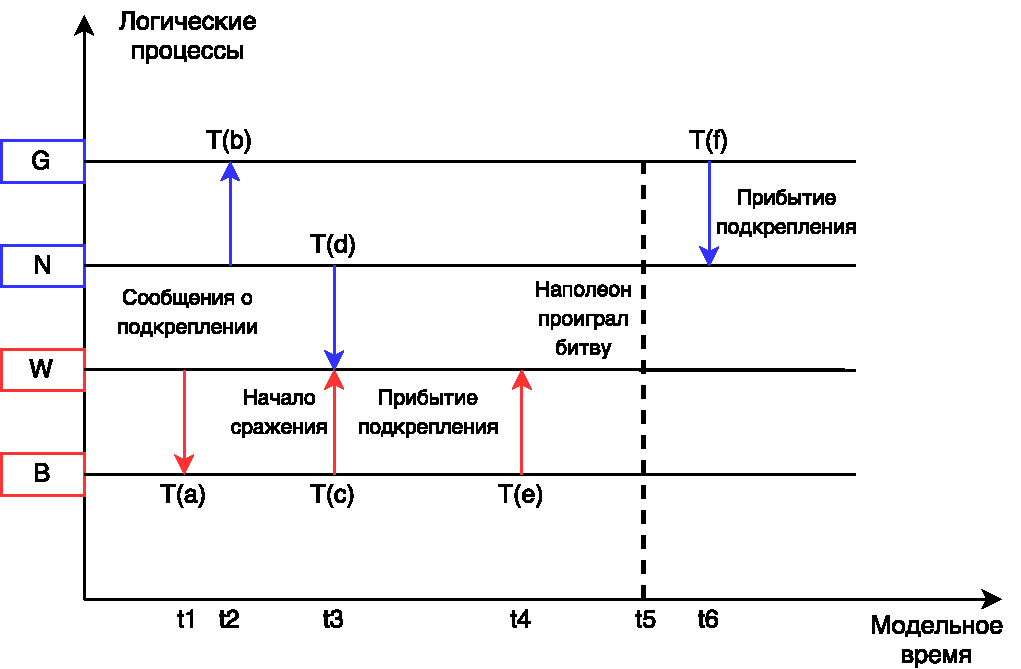
\includegraphics[scale=1]{images/waterloo.pdf}
\caption{Корректная временная диаграмма исполнения модели}
\label{fig:Корректная временная диаграмма исполнения модели}
\end{figure}

Наполеон Бонапарт (процесс $N$) должен был вступить в бой с герцогом Веллингтоном (процесс $W$), расположившемся со своей английской армией на пути к Брюсселю. Но оба полководца ждали подкрепления: герцог Веллингтон --- прусского князя Блюхера (процесс $B$), Наполеон --- своего маршала Груш\'и (процесс $G$). И Наполеон и Веллингтон отправили командующим своими подкреплениями сообщения с категорическим требованием скорейшего прибытия под Ватерлоо для усиления основной группировки войск. Тем временем, армия Бонапарта в ожидании прибытия подкрепления маршала Груши начала атаку неприятеля. Веллингтону ничего не оставалось, как принять бой. Не смотря на более выгодное расположение войск Веллингтона и примерно равные силы с Наполеоном, французы развивали успешное наступление на англичан и едва не опрокинули их --- положение Веллингтона становилось критическим. И только вовремя подоспевшее подкрепление князя Блюхера помогло герцогу сдержать натиск Наполеона, а затем и перейти в контрнаступление на французов. После чего, так и не дождавшийся своего маршала с подкреплением, французский император был разбит.

Предположим, что эти процессы выполняются на распределенной системе. И логический процесс $B$ в силу определенных причин (например, резко возросла нагрузка на процессор) выполняется медленнее. Следовательно возникли задержки. Для логического процесса $W$ получение сообщения в момент времени $t5$ означает изменение прошлого в момент времени $t4$, что нарушает корректную последовательность развития моделирования, рисунок~\ref{fig:Некорректная временная диаграмма исполнения модели}.

\begin{figure}[!ht]
\centering
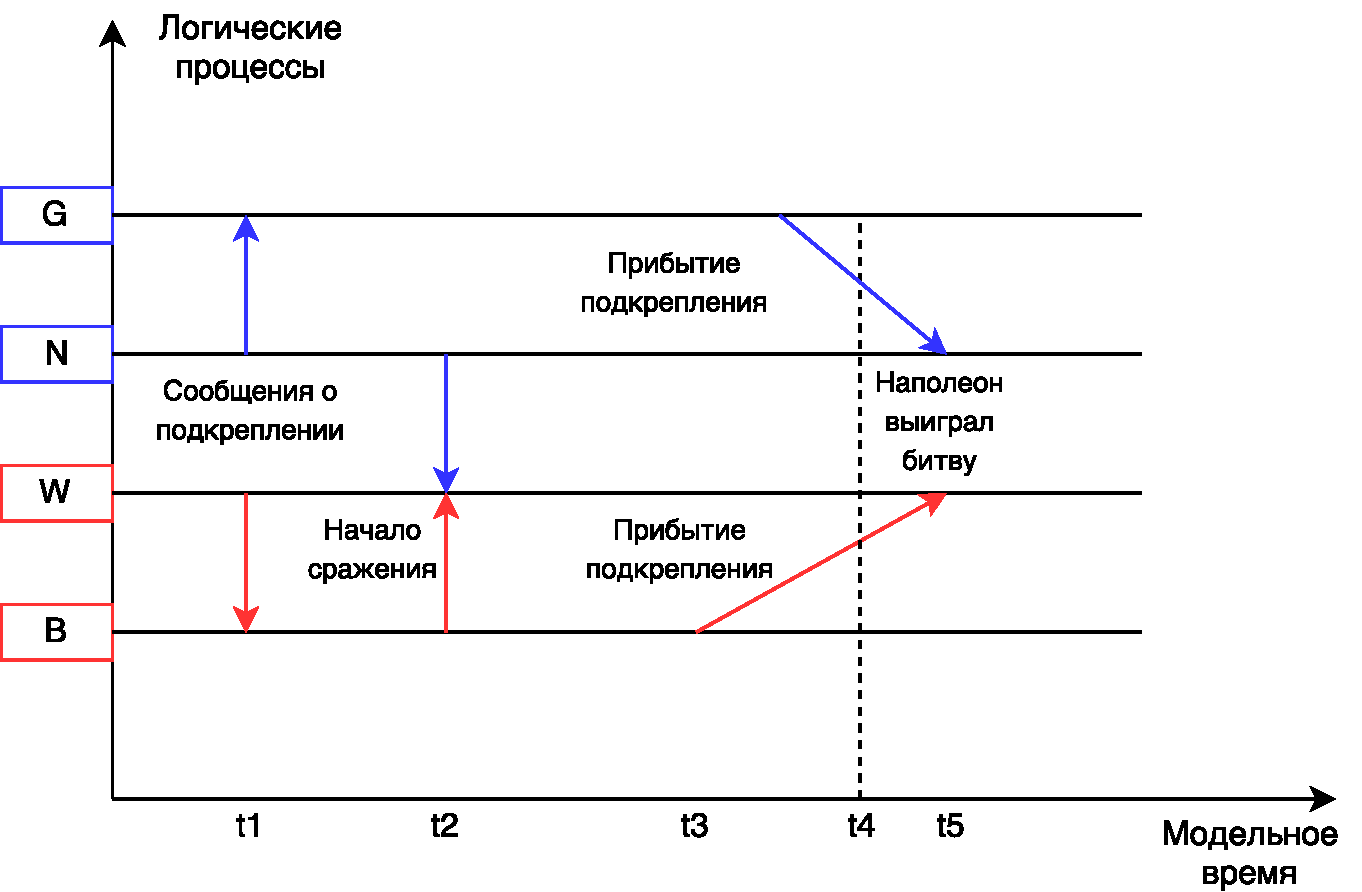
\includegraphics[scale=1]{images/unwaterloo.pdf}
\caption{Некорректная временная диаграмма исполнения модели}
\label{fig:Некорректная временная диаграмма исполнения модели}
\end{figure}

Для того, чтобы модель правильно воспроизводила последовательность событий в моделируемой системе, необходимо чтобы не возникало подобных парадоксов времени.
Тот процесс продвигает свое время вперед, который получил сообщение от процесса с б\'ольшим временем. Если процесс получает сообщение от процесса с меньшим временем, т.е. $t_i^m<t_i^n, \, m \to n$, получаем парадокс, т.е. говорят, что процесс приславший сообщение \elki{из прошлого} отстает во времени~\cite{okol}.

Для того, чтобы парадоксов времени в системе не возникало, необходимо предусмотреть специальные программы, которые бы синхронизировали по времени процессы в моделируемой системе. Такие программы получили название алгоритмов синхронизации модельного времени. Алгоритмы синхронизации разнообразны, но все их как правило можно разделить на два основных класса: консервативные и оптимистические.

Если синхронизация модельного времени процессов происходит под управлением консервативного алгоритма, это предполагает, что процесс получает сообщения в том же порядке, в котором их посылает ему отправитель.
Иначе, консервативные алгоритмы блокируют продвижение модельного времени в том случае, если процесс получил сообщение от процесса с меньшим временем.

Оптимистические алгоритмы в аналогичном случае осуществляют откат времени процесса с большим временем до времени процесса, приславшего сообщение, обрабатывает его, а так же заново обрабатывают все сообщения от этого времени до текущего в правильной временной последовательности.

%\newpage
%============================================================================================================================

\section{Ссылки} \label{sect1_2}
Сошлёмся на библиографию. Одна ссылка: \cite[с.~54]{Sokolov}\cite[с.~36]{Gaidaenko}. Две ссылки: \cite{Sokolov,Gaidaenko}. Много ссылок:  \cite[с.~54]{Lermontov,Management,Borozda} \cite{Lermontov,Management,Borozda,Marketing,Constitution,FamilyCode,Gost.7.0.53,Razumovski,Lagkueva,Pokrovski,Sirotko,Lukina,Methodology,Encyclopedia,Nasirova,Berestova,Kriger}. И ещё немного ссылок: \cite{Article,Book,Booklet,Conference,Inbook,Incollection,Manual,Mastersthesis,Misc,Phdthesis,Proceedings,Techreport,Unpublished}. \cite{medvedev2006jelektronnye, CEAT:CEAT581, doi:10.1080/01932691.2010.513279,Gosele1999161,Li2007StressAnalysis, Shoji199895,test:eisner-sample,AB_patent_Pomerantz_1968,iofis_patent1960}

%Попытка реализовать несколько ссылок на конкретные страницы для стандартной реализации:[\citenum{Sokolov}, с.~54; \citenum{Gaidaenko}, с.~36].

%Несколько источников мультицитата \cites[vii--x, 5, 7]{Sokolov}[v--x, 25, 526]{Gaidaenko} поехали дальше

Ссылки \nom[]{ОЛОЛ}{Это ссылки конечно же.} на собственные работы:~\cite{vakbib1, confbib1}

Сошлёмся на приложения: Приложение \ref{AppendixA}, Приложение \ref{AppendixB2}.

Сошлёмся на формулу: формула \eqref{eq:equation1}.

Сошлёмся на изображение: рисунок \ref{img:knuth}.
Имитационное моделирование систем --- искусство и наука. \cite{Shennon}

%\newpage
%============================================================================================================================

\section{Формулы} \label{sect1_3}

Благодаря пакету \textit{icomma}, \LaTeX~одинаково хорошо воспринимает в качестве десятичного разделителя и запятую ($3,1415$), и точку ($3.1415$).

\subsection{Ненумерованные одиночные формулы} \label{subsect1_3_1}

Вот так может выглядеть формула \nom[]{НИИИ}{Формула такая формула, ололо}, которую необходимо вставить в строку по тексту: $x \approx \sin x$ при $x \to 0$.

А вот так выглядит ненумерованая отдельностоящая формула \Gls{math} c подстрочными и надстрочными индексами:
\[
(x_1+x_2)^2 = x_1^2 + 2 x_1 x_2 + x_2^2
\]

При использовании дробей формулы могут получаться очень высокие:
\[
  \frac{1}{\sqrt{2}+
  \displaystyle\frac{1}{\sqrt{2}+
  \displaystyle\frac{1}{\sqrt{2}+\cdots}}}
\]

В формулах можно использовать греческие буквы:
\[
\alpha\beta\gamma\delta\epsilon\varepsilon\zeta\eta\theta\vartheta\iota\kappa\lambda\\mu\nu\xi\pi\varpi\rho\varrho\sigma\varsigma\tau\upsilon\phi\varphi\chi\psi\omega\Gamma\Delta\Theta\Lambda\Xi\Pi\Sigma\Upsilon\Phi\Psi\Omega
\]

\def\slantfrac#1#2{ \hspace{3pt}\!^{#1}\!\!\hspace{1pt}/
  \hspace{2pt}\!\!_{#2}\!\hspace{3pt}
} %Макрос для красивых дробей в строчку (например, 1/2)
Для красивых дробей (например, в индексах) можно добавить макрос
\verb+\slantfrac+ и писать $\slantfrac{1}{2}$ вместо $1/2$.
%\newpage
%============================================================================================================================

\subsection{Ненумерованные многострочные формулы} \label{subsect1_3_2}

Вот так можно написать две формулы, не нумеруя их, чтобы знаки равно были строго друг под другом:
\begin{align}
  f_W & =  \min \left( 1, \max \left( 0, \frac{W_{soil} / W_{max}}{W_{crit}} \right)  \right), \nonumber \\
  f_T & =  \min \left( 1, \max \left( 0, \frac{T_s / T_{melt}}{T_{crit}} \right)  \right), \nonumber
\end{align}

Выровнять систему ещё и по переменной $ x $ можно, используя окружение \verb|alignedat| из пакета \verb|amsmath|. Вот так: 
\[
    |x| = \left\{
    \begin{alignedat}{2}
        &&x, \quad &\text{eсли } x\geqslant 0 \\
        &-&x, \quad & \text{eсли } x<0
    \end{alignedat}
    \right.
\]
Здесь первый амперсанд  означает выравнивание по~левому краю, второй "--- по~$ x $, а~третий "--- по~слову <<если>>. Команда \verb|\quad| делает большой горизонтальный пробел. 

Ещё вариант:
\[
    |x|=
    \begin{cases}
    \phantom{-}x, \text{если } x \geqslant 0 \\
    -x, \text{если } x<0
    \end{cases}
\]

Кроме того, для  нумерованых формул \verb|alignedat|  делает вертикальное
выравнивание номера формулы по центру формулы. Например,  выравнивание компонент вектора:
\begin{equation}
 \label{eq:2p3}
 \begin{alignedat}{2}
{\mathbf{N}}_{o1n}^{(j)} = \,{\sin} \phi\,n\!\left(n+1\right)
         {\sin}\theta\,
         \pi_n\!\left({\cos} \theta\right)
         \frac{
               z_n^{(j)}\!\left( \rho \right)
              }{\rho}\,
           &{\boldsymbol{\hat{\mathrm e}}}_{r}\,+   \\
+\,
{\sin} \phi\,
         \tau_n\!\left({\cos} \theta\right)
         \frac{
            \left[\rho z_n^{(j)}\!\left( \rho \right)\right]^{\prime}
              }{\rho}\,
            &{\boldsymbol{\hat{\mathrm e}}}_{\theta}\,+   \\
+\,
{\cos} \phi\,
         \pi_n\!\left({\cos} \theta\right)
         \frac{
            \left[\rho z_n^{(j)}\!\left( \rho \right)\right]^{\prime}
              }{\rho}\,
            &{\boldsymbol{\hat{\mathrm e}}}_{\phi}\:.
\end{alignedat}
\end{equation}

Ещё об отступах. Иногда для лучшей "читаемости" формул полезно
немного исправить стандартные интервалы \LaTeX с учётом логической
структуры самой формулы. Например в формуле~\ref{eq:2p3} добавлен
небольшой отступ \verb+\,+ между основными сомножителями, ниже
результат применения всех вариантов отступа:
\begin{align*}
\backslash! &\quad f(x) = x^2\! +3x\! +2 \\
  \mbox{по-умолчанию} &\quad f(x) = x^2+3x+2 \\
\backslash, &\quad f(x) = x^2\, +3x\, +2 \\
\backslash{:} &\quad f(x) = x^2\: +3x\: +2 \\
\backslash; &\quad f(x) = x^2\; +3x\; +2 \\
\backslash \mbox{space} &\quad f(x) = x^2\ +3x\ +2 \\
\backslash \mbox{quad} &\quad f(x) = x^2\quad +3x\quad +2 \\
\backslash \mbox{qquad} &\quad f(x) = x^2\qquad +3x\qquad +2
\end{align*}


Можно использовать разные математические алфавиты:
\begin{align}
\mathcal{ABCDEFGHIJKLMNOPQRSTUVWXYZ} \nonumber \\
\mathfrak{ABCDEFGHIJKLMNOPQRSTUVWXYZ} \nonumber \\
\mathbb{ABCDEFGHIJKLMNOPQRSTUVWXYZ} \nonumber
\end{align}

Посмотрим на систему уравнений на примере аттрактора Лоренца:

\[ 
\left\{
  \begin{array}{rl}
    \dot x = & \sigma (y-x) \\
    \dot y = & x (r - z) - y \\
    \dot z = & xy - bz
  \end{array}
\right.
\]

А для вёрстки матриц удобно использовать многоточия:
\[ 
\left(
  \begin{array}{ccc}
  	a_{11} & \ldots & a_{1n} \\
  	\vdots & \ddots & \vdots \\
  	a_{n1} & \ldots & a_{nn} \\
  \end{array}
\right)
\]


%\newpage
%============================================================================================================================
\subsection{Нумерованные формулы} \label{subsect1_3_3}

А вот так пишется нумерованая формула:
\begin{equation}
  \label{eq:equation1}
  e = \lim_{n \to \infty} \left( 1+\frac{1}{n} \right) ^n
\end{equation}

Нумерованых формул может быть несколько:
\begin{equation}
  \label{eq:equation2}
  \lim_{n \to \infty} \sum_{k=1}^n \frac{1}{k^2} = \frac{\pi^2}{6}
\end{equation}

Впоследствии на формулы (\ref{eq:equation1}) и (\ref{eq:equation2}) можно ссылаться.

Сделать так, чтобы номер формулы стоял напротив средней строки, можно, используя окружение \verb|multlined| (пакет \verb|mathtools|) вместо \verb|multline| внутри окружения \verb|equation|. Вот так:
\begin{equation} % \tag{S} % tag - вписывает свой текст 
  \label{eq:equation3}
    \begin{multlined}
        1+ 2+3+4+5+6+7+\dots + \\ 
        + 50+51+52+53+54+55+56+57 + \dots + \\ 
        + 96+97+98+99+100=5050 
    \end{multlined}
\end{equation}

Используя команду \verb|\labelcref| из пакета \verb|cleveref|, можно
красиво ссылаться сразу на несколько формул
(\labelcref{eq:equation1,eq:equation3,eq:equation2}), даже перепутав
порядок ссылок \verb|(\labelcref{eq:equation1,eq:equation3,eq:equation2})|.

